\section{Exercise 4 - Binary Tree Algorithms for \texttt{MPI\_Bcast} and \texttt{MPI\_Reduce}}
Instead of “lined up” processes we now want to use a binary tree structure and according algorithms 
\texttt{MY\_Reduce\_T()} and \texttt{MY\_Bcast\_T()} for reduction and broadcasting. As we understand 
each process as a node, we will use the wording node from now on. For indexing of the nodes, we use preorder traversal.

We start very similar to the implementations of \texttt{MY\_Reduce\_P()} and \texttt{MY\_Bcast\_P()} 
from exercise 2. For the reduction \texttt{MY\_Reduce\_P()}  the root node (rank $=0$) on level 0 should 
gain the reduced result. Hence, the leaves start by sending the data block by block to their parents. All 
interior nodes receive exactly two data blocks per communication round. One from their left and one from their 
right child. After performing a local reduction, the data is sent to the nodes parent. In the end, the root 
node receives the data from its two children and ends up with the reduction result. For the broadcast 
\texttt{MY\_Bcast\_P()}, the root node sends the data block wise to its two children. A child receives 
the data and immediately forwards this data to its children, in case it is not a leaf.\\

The trivial combination of \texttt{MY\_Reduce\_T()} and \texttt{MY\_Bcast\_T()} can be seen 
as a pipelined variant of \texttt{MPI\_Allreduce()}.\\

\begin{figure}[h]
    \begin{center}
        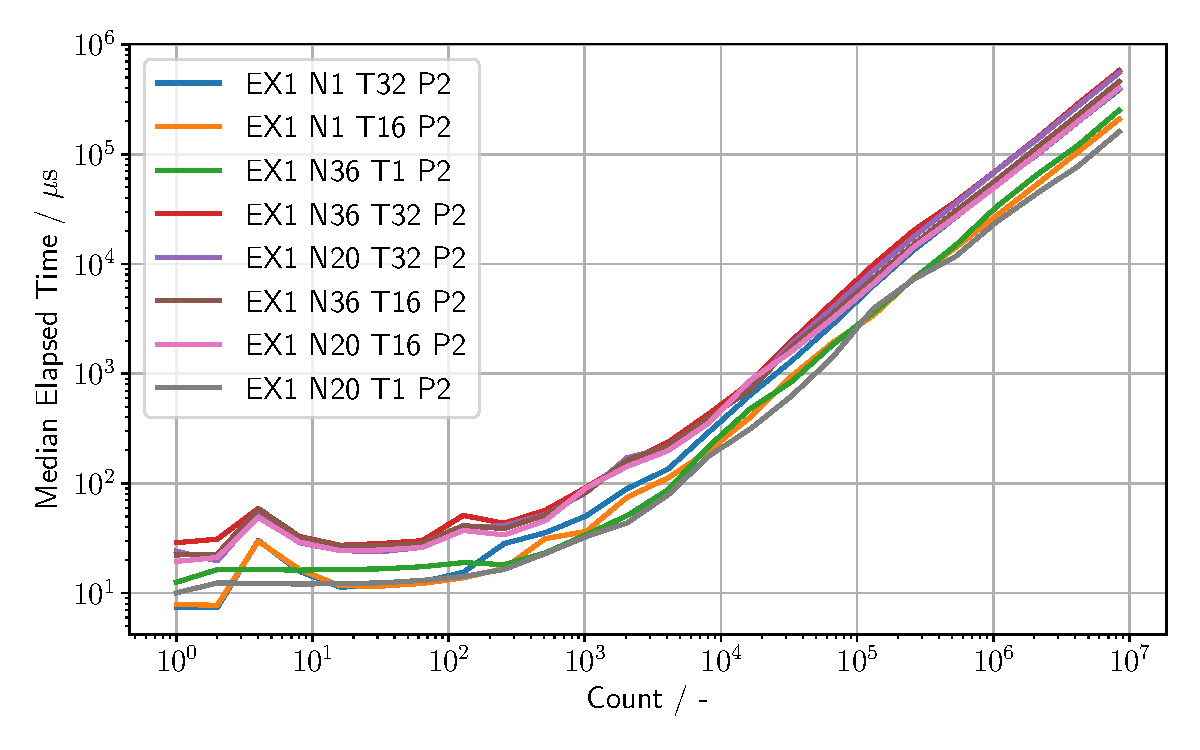
\includegraphics[width= 0.88\linewidth]{figures/Ex1_2.pdf} 
        \label{ref_plot_task_5}
        \caption{Benchmark both algorithms - \texttt{yarg32()} is faster than \texttt{yarg()} for all feasible values of $d$}
    \end{center}
\end{figure}
\pagebreak

\section{Exercise 5 - Integrated, Improved Binary Tree Algorithm}
We aim to devise an integrated, improved binary tree algorithm for \texttt{MPI\_Allreduce()}. Our 
implementation \texttt{MY\_Allreduce\_T()} is based on the algorithm for a doubly pipelined binary 
tree described in [Jesper Larsson Träff. A doubly-pipelined, dual-root reduction-to-all algorithm and 
implementation. arXiv:2109.12626, 2021.]. Note that we use only one tree, so there will never happen any 
communication between roots of different trees, as there is no. Per communication round, the reduction of 
one block can be performed. Hence, for complete reduction as much communication rounds are needed, 
as there are blocks. The idea is, that the root node starts with its broadcast-like send operations 
as soon as it received the data of the first block. The root node performs a local reduction against 
its own value and then the broadcasting starts while other blocks are still (or not yet) 
in their reduction phase. \\


\pagebreak
\section{Exercise 6 - Improvement with Sibling Leave Communication (BONUS)}
Not implemented.

\section{Exercise 7 - Implemenetation and Benchmarking of Improved Version (BONUS)}
Not implemented.
\pagebreak